\section{Vision par ordinateur}\label{sec:vision}

\subsection{Objectif}

La couverture nuageuse est une variable clé pour la caractérisation du
rayonnement solaire reçu par la surface de la mer. Les capteurs commerciaux
de nébulosité (pyranomètres, détecteurs infrarouge) sont coûteux et peu adaptés
à une intégration compacte dans une station embarquée. Une approche par vision
par ordinateur a donc été explorée comme alternative bas coût, en s'appuyant
sur la caméra déjà présente sur le PCB étage 2.

\subsection{Méthode : segmentation par seuillage HSV}

La caméra \textit{Joy-it ESP32} est orientée vers le zénith sous le dôme en
plexiglas. Elle capture des images périodiques du ciel. L'algorithme de
traitement repose sur une segmentation en deux étapes :

\begin{enumerate}
  \item \textbf{Conversion HSV.} L'image RGB est convertie dans l'espace
    colorimétrique HSV (Teinte, Saturation, Valeur). Cet espace sépare
    l'information de couleur (teinte) de la luminosité (valeur) et de la
    pureté de la couleur (saturation), ce qui le rend plus robuste aux
    variations d'exposition que le RVB direct.

  \item \textbf{Seuillage.} Les nuages, plus blancs et moins saturés que le
    ciel bleu, sont isolés par un masque combinant une saturation basse et
    une valeur élevée. Le seuil est déterminé empiriquement sur un ensemble
    d'images représentatives de différentes conditions météorologiques.
\end{enumerate}

Le taux de couverture nuageuse est calculé comme le rapport entre le nombre
de pixels classés ``nuage'' et le nombre total de pixels de l'image, après
exclusion des bords occupés par le boîtier.

\begin{figure}[H]
  \centering
  \begin{subfigure}[b]{0.48\textwidth}
    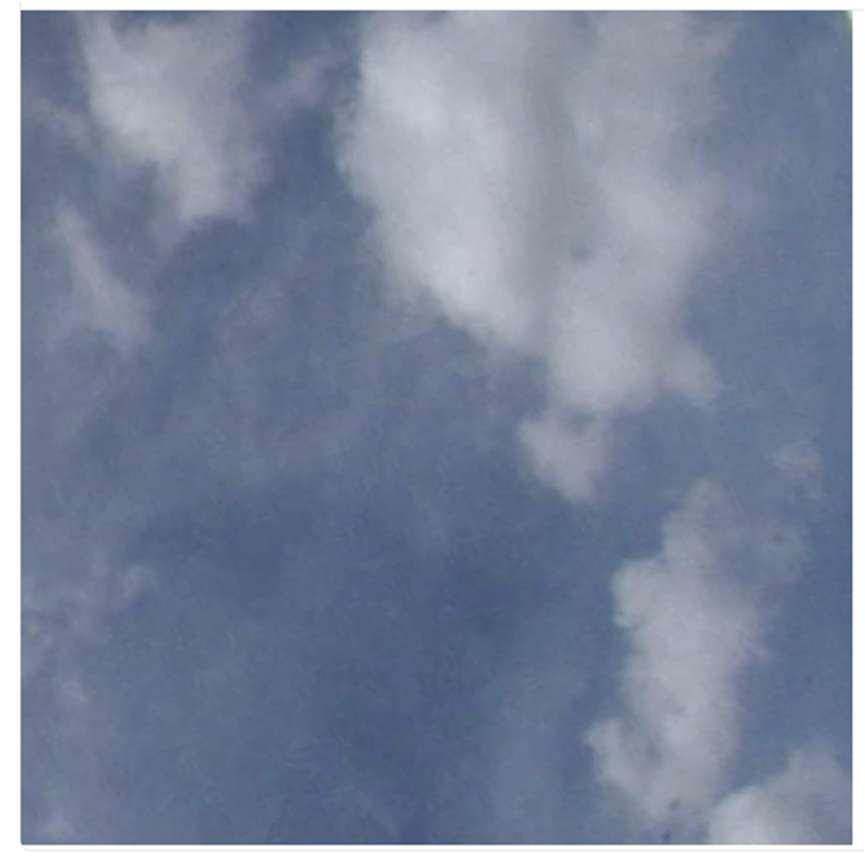
\includegraphics[width=\textwidth]{images/vision_ciel.png}
    \caption{Image brute du ciel}
  \end{subfigure}
  \hfill
  \begin{subfigure}[b]{0.48\textwidth}
    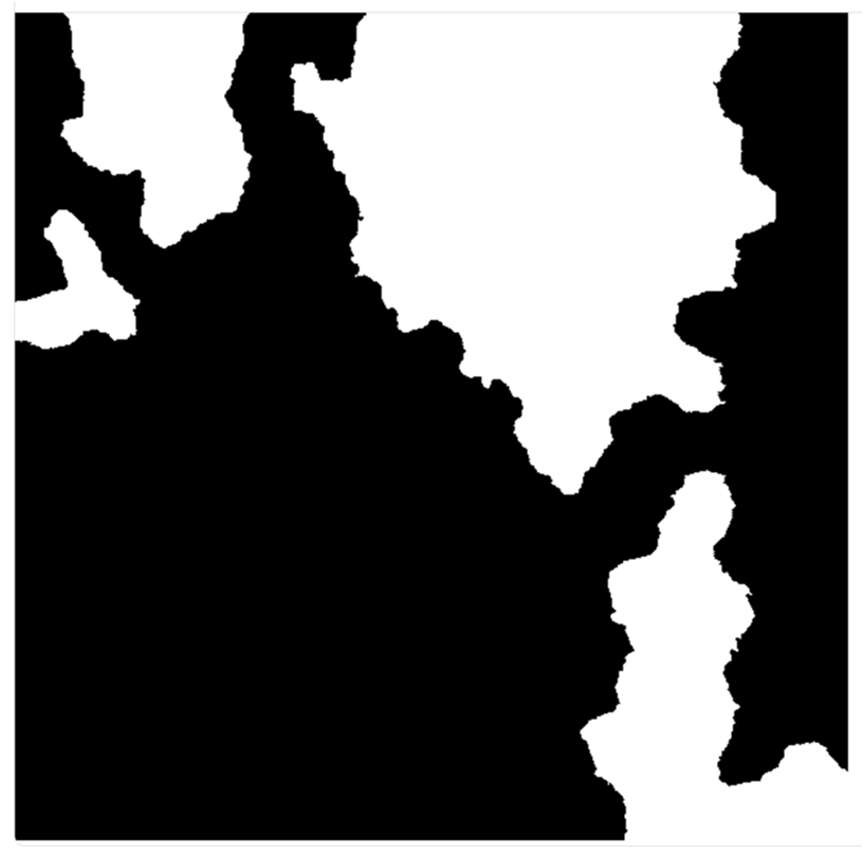
\includegraphics[width=\textwidth]{images/vision_masque.png}
    \caption{Masque binaire (blanc = nuage)}
  \end{subfigure}
  \caption{Exemple de segmentation nuages/ciel par seuillage HSV.}
  \label{fig:cv_segmentation}
\end{figure}

\subsection{Résultats et perspectives}

Les tests préliminaires montrent que l'algorithme discrimine correctement
les nuages blancs sur fond de ciel bleu dans des conditions standard
(figure~\ref{fig:cv_segmentation}). Plusieurs cas difficiles restent à traiter :

\begin{itemize}
  \item \textbf{Ciel uniformément couvert} : sans contraste bleu/blanc,
    le seuillage par saturation devient peu fiable.
  \item \textbf{Coucher et lever de soleil} : la teinte du ciel vire
    vers l'orange/rouge, perturbant le masque basé sur la teinte bleue.
  \item \textbf{Éblouissement direct} : lorsque le soleil entre dans
    le champ de la caméra, la surexposition locale crée de faux positifs.
\end{itemize}

Pour améliorer la robustesse, deux pistes sont envisagées : l'adaptation
dynamique du seuil en fonction de l'heure et de la position GPS (azimut
solaire calculé), et l'entraînement d'un classifieur léger (réseau de
neurones convolutionnel de petite taille ou k-means sur l'histogramme HSV)
utilisable sur le microcontrôleur ESP32 ou sur l'ordinateur de bord.
